\documentclass[11pt]{article}

\usepackage{graphicx}

\begin{document}
\title{Comparison of symmetric ciphers in OpenSSL \\ \large HW1 - CNS Sapienza}
\author{Matteo Salvino 1708108}
\date{04 November 2019}
\maketitle

\section{Goals}
For the first CNS's homework we have to reach several goals in order to understand deeply how ciphers and mode of operations works together. First of all, we start to compare some different symmetric ciphers in terms of encryption/decryption speed. Subsequently, we pick a pair (cipher, operation mode) to check if encryption process require more or less time than decryption process. In particular, we will need to define a ratio called average speed ratio that is given by :
\begin{center}
$\frac{average\hspace{0.1cm}speed\hspace{0.1cm}of\hspace{0.1cm}encryption}{average\hspace{0.1cm}speed\hspace{0.1cm}of\hspace{0.1cm}decryption}$
\end{center}
Finally, we will report how changing operation mode/cipher/file size affect speed of encryption/decryption process and speed ratio, building a graphical representation of results.
\section{Comparison Environment}
To compare different symmetric ciphers, we will use a python library called \textbf{cryptography}, which is based on OpenSSL interface. For our experiments we will use several sample files with different size (greater than 100KB), which are generated by the following python function :
\begin{center}
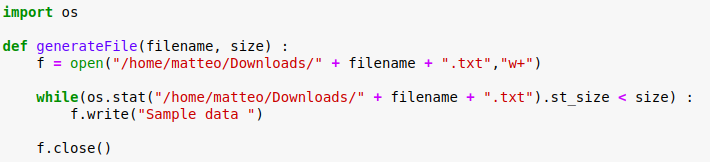
\includegraphics[scale=0.4]{./file_factory.png}
\end{center}
In this experiment we will consider four symmetric ciphers (Blowfish, 3DES, AES, IDEA), and two mode of operations (ECB, CBC). Now, let's see how different symmetric ciphers behave in terms of speed in MB/s. An important note to take in consideration is that since the time required for encryption/decryption process depends on system's available resources, each process will be executed five times and the corresponding average execution time will be the arithmetic mean of times obtained in these executions. Hence, we define the speed in the following way :
\begin{center}
speed = $\frac{|file|}{average\hspace{0.1cm}execution\hspace{0.1cm}time}$ 
\end{center}
In order to perform encryption we will use a small python function :
\begin{center}
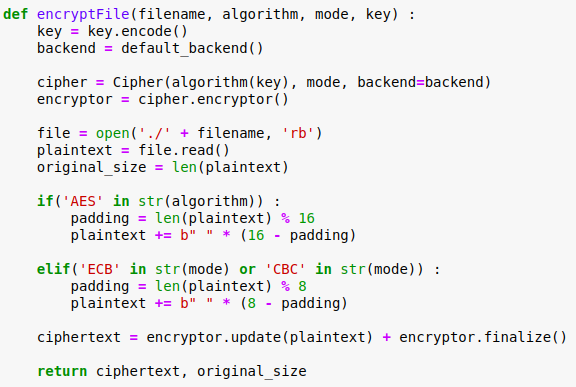
\includegraphics[scale=0.5]{./encryption_function.png}
\end{center}
This function takes as input a filename, the cipher, mode of operation and a key. Subsequently, the key (a string in this case) will be encoded to assume a byte form. Then the cipher is initialized with given input parameters, the file is read in a variable, and some particular case will be managed (eventually adding some padding bits). Finally, encryption function is called and the corresponding ciphertext is returned. We also return the original size of the file we have read, in order to reconstruct the original file removing the padding bits. The function that we use for perform decryption is very similar to the previous one :
\begin{center}
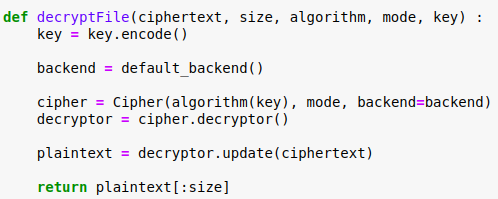
\includegraphics[scale=0.5]{./decryption_function.png}
\end{center}
To get the execution time of encryption/decryption processes, we wrap the previous functions with this code :
\begin{center}
start\_time = time.time() \\
function() \\
exec\_time = time.time() - start\_time \\ 
\end{center}
So far we have seen how is constituted our environment, but time has came to talk about his significant factors.
\subsection{Significant Factors}
In this section we want to cover a key concept that is represented by the relationship between symmetric ciphers and mode of operations. In order to understand how they work together we should answer to the following questions :
\begin{itemize}
\item How changing the operating mode affects speed and speed ratio ?
\item How changing the cipher affects speed and speed ratio ?
\item How changing the file size affects speed and speed ratio ?
\end{itemize}
First of all we need to think about mode of operations available for this experiment. For ECB, we known that the plaintext will be subdivided in block of a certain size, to the last block eventually will add some bits as padding, and these blocks will be encrypted with a given key k. Each block will be encrypted with the same key k, so we could encrypt several plaintext blocks in parallel, reducing the time required for encryption process. For decryption, since these blocks are independent each other, they can decrypted in parallel, having as a consequence a time reduction for decryption process. An important question to ask yourself is the following : Is it possible to perform some preprocessing in order to further reduce the time required by encryption and decryption process ? The answer is no, because we can't see some preprocessing to apply. Now, we consider CBC, and from the theory we know that plaintext is subdivided in block of certain size (as ECB), but each block, except the first block, is encrypted xoring itself with the previous ciphertext block. The first one is encrypted by xoring itself with a given seed (also called initialization vector). We can simply conclude that in this case we can't parallelize encryption process, because each block, except the first one, depends on the previous one, so we can proceed only in sequential way. However, we can parallelize the decryption process because for construct a plaintext block we need to have the corresponding ciphertext block and the previous one, but at this point we have available all ciphertext blocks. Can i do some preprocessing in order to speed up encryption/decryption process ? The answer is again no, because we can't see any preprocessing to apply.
\subsection{Blowfish}
After a brief pros and cons description of modes of operation, lets start considering a pair (cipher, mode of operation), where we choose Blowfish as cipher and ECB as mode of operation (initially). Next we will compute the speed of encryption and decryption process for each mode of operation. We summarize the results obtained for each mode in the following table :
\begin{center}
\begin{tabular}{| c | c | c | c |}
\hline
\multicolumn{4}{|c|}{Blowfish (file01.txt)} \\
\hline
Mode & Encryption (MB/s) & Decryption (MB/s) & Speed ratio\\
\hline
ECB & 1.7026 & 1.9766 & 0.8613 \\
\hline
CBC & 1.8329 & 2.0829 & 0.8799 \\
\hline
\end{tabular}
\end{center}
To answer to the third question, we generate four file (file01.txt, file1.txt, file10.txt and file100.txt) with size respectively 100KB, 1MB, 10MB and 100MB. Then to understand how the file size can affect encryption/decryption speed and thus the speed ratio, we will compute the time required for encryption and decryption process for Blowfish with ECB for each operating mode for each file. The results can be summarized in the following table
\begin{center}
\begin{tabular}{| c | c | c | c |}
\hline
\multicolumn{4}{|c|}{Blowfish-ECB} \\
\hline
File & Encryption (MB/s) & Decryption (MB/s) & Speed ratio\\
\hline
file1.txt & 3.9806 & 4.4552 & 0.8934 \\
\hline
file10.txt & 4.2256 & 4.6577 & 0.9072 \\
\hline
file100.txt & 3.9846 & 4.1454 & 0.9611 \\
\hline
\end{tabular}
\end{center}
\pagebreak and shown in the following plots :
\begin{center}
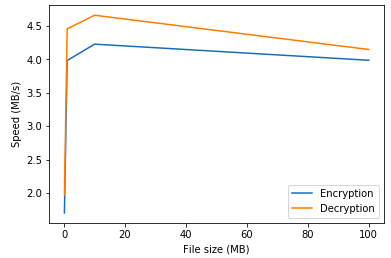
\includegraphics[scale=0.5]{./enc_dec_speed_blowfish_ecb.png}
\end{center}
We can see that when a file have a certain size the environment exploits in optimal way all his core, but when the file size is huge, then the cpu is forced to wait that a working thread became free. These results has a consequence over the average speed ratio, as reported in the plot below 
\begin{center}
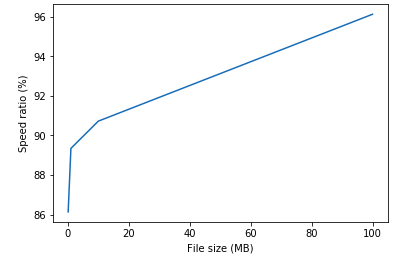
\includegraphics[scale=0.6]{./avg_speed_ratio_blowfish_ecb.png}
\end{center}
This trend is justified by the fact that the decryption speed when the file size changes is more affected than the encryption speed, so the ratio begins to grow.\\\\ Presently, we will repeat this procedure for Blowfish in CBC mode. The results obtained are the following
\begin{center}
\begin{tabular}{| c | c | c | c |}
\hline
\multicolumn{4}{|c|}{Blowfish-CBC} \\
\hline
File & Encryption (MB/s) & Decryption (MB/s) & Speed ratio\\
\hline
file1.txt & 3.8727 & 4.8097 & 0.8051 \\
\hline
file10.txt & 4.0246 & 4.944 & 0.8140 \\
\hline
file100.txt & 3.8623 & 4.4073 & 0.8763 \\
\hline
\end{tabular}
\end{center}
and shown in the following plots :
\begin{center}
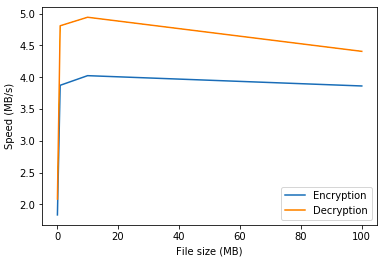
\includegraphics[scale=0.45]{./enc_dec_speed_blowfish_cbc.png}
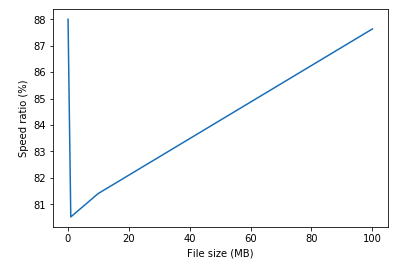
\includegraphics[scale=0.45]{./avg_speed_ratio_blowfish_cbc.png}
\end{center}
\subsection{TripleDES}
Now we choose TripleDES as cipher and ECB as mode of operation (initially). We summarize the results obtained for each mode in the following table :
\begin{center}
\begin{tabular}{| c | c | c | c |}
\hline
\multicolumn{4}{|c|}{TripleDES (file01.txt)} \\
\hline
Mode & Encryption (MB/s) & Decryption (MB/s) & Speed ratio\\
\hline
ECB & 0.6731 & 0.7429 & 0.9060 \\
\hline
CBC & 0.7374 & 0.8188 & 0.9006 \\
\hline
\end{tabular}
\end{center}
Lets analyze how the encryption/decryption speed and the average speed ratio is affects by the file size (in ECB mode) :
\begin{center}
\begin{tabular}{| c | c | c | c |}
\hline
\multicolumn{4}{|c|}{TripleDES-ECB} \\
\hline
File & Encryption (MB/s) & Decryption (MB/s) & Speed ratio\\
\hline
file1.txt & 1.006 & 1.0205 & 0.9858 \\
\hline
file10.txt & 1.0271 & 1.0517 & 0.9766 \\
\hline
file100.txt & 1.0158 & 1.0196 & 0.9963 \\
\hline
\end{tabular}
\end{center}
and shown in the plots below :
\begin{center}
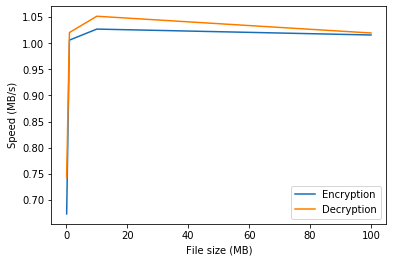
\includegraphics[scale=0.4]{./enc_dec_speed_3des_ecb.png}
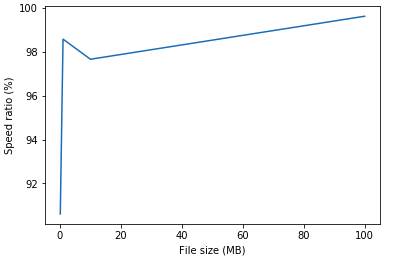
\includegraphics[scale=0.4]{./avg_speed_ratio_3des_ecb.png}
\end{center}
Now, we will repeat this procedure for CBC mode of operation. The results can be summarized in the following table :
\begin{center}
\begin{tabular}{| c | c | c | c |}
\hline
\multicolumn{4}{|c|}{TripleDES-CBC} \\
\hline
File & Encryption (MB/s) & Decryption (MB/s) & Speed ratio\\
\hline
file1.txt & 0.9684 & 1.0145 & 0.9545 \\
\hline
file10.txt & 1.0299 & 1.0645 & 0.9674 \\
\hline
file100.txt & 0.9848 & 1.014 & 0.9711 \\
\hline
\end{tabular}
\end{center}
and seen in these plots :
\begin{center}
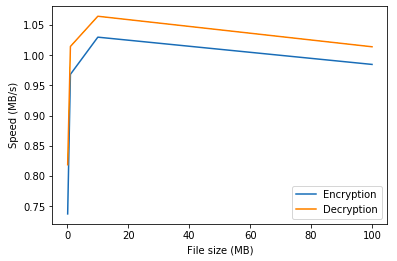
\includegraphics[scale=0.45]{./enc_dec_speed_3des_cbc.png}
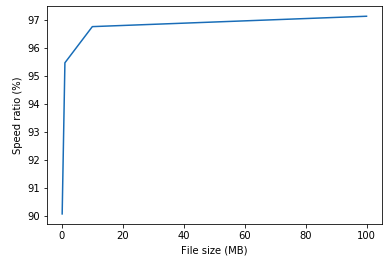
\includegraphics[scale=0.45]{./avg_speed_ratio_3des_cbc.png}
\end{center}
\subsection{AES}
Another cipher in our experiment is AES with a key length of 128 bits and ECB as mode of operation (initially). The results are summarized in the table below :
\begin{center}
\begin{tabular}{| c | c | c | c |}
\hline
\multicolumn{4}{|c|}{AES (file01.txt)} \\
\hline
Mode & Encryption (MB/s) & Decryption (MB/s) & Speed ratio\\
\hline
ECB & 3.6834 & 5.2243 & 0.7050 \\
\hline
CBC & 4.5245 & 5.6991 & 0.7938 \\
\hline
\end{tabular}
\end{center}
Currently, we analyze how AES in ECB mode behave for several file size. The results are reported in the following table :
\begin{center}
\begin{tabular}{| c | c | c | c |}
\hline
\multicolumn{4}{|c|}{AES-ECB} \\
\hline
File & Encryption (MB/s) & Decryption (MB/s) & Speed ratio\\
\hline
file1.txt & 21.3935 & 38.7758 & 0.5517 \\
\hline
file10.txt & 23.5947 & 49.6866 & 0.4748\\
\hline
file100.txt & 14.9159 & 18.7279 & 0.7964 \\
\hline
\end{tabular}
\end{center}
and shown in the plots below :
\begin{center}
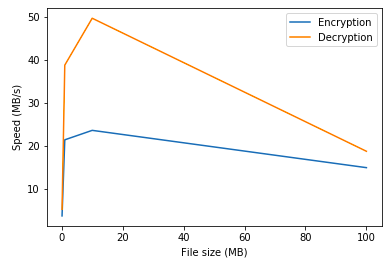
\includegraphics[scale=0.45]{./enc_dec_speed_aes_ecb.png}
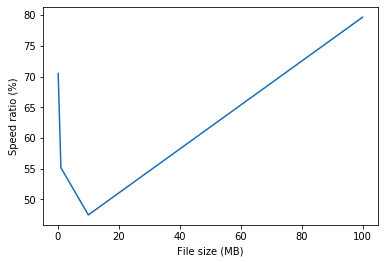
\includegraphics[scale=0.45]{./avg_speed_ratio_aes_ecb.png}
\end{center}
Whereas for AES in CBC mode, we obtain these results :
\begin{center}
\begin{tabular}{| c | c | c | c |}
\hline
\multicolumn{4}{|c|}{AES-CBC} \\
\hline
File & Encryption (MB/s) & Decryption (MB/s) & Speed ratio\\
\hline
file1.txt & 16.8822 & 55.9708 & 0.3016 \\
\hline
file10.txt & 15.2455 & 39.184 & 0.3890 \\
\hline
file100.txt & 10.7694 & 16.6241 & 0.6478 \\
\hline
\end{tabular}
\end{center}
\begin{center}
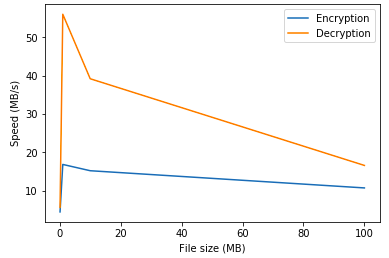
\includegraphics[scale=0.45]{./enc_dec_speed_aes_cbc.png}
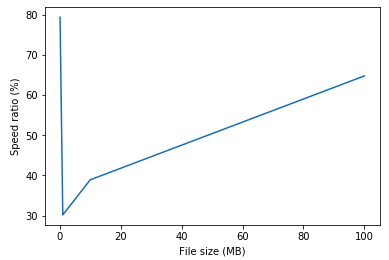
\includegraphics[scale=0.45]{./avg_speed_ratio_aes_cbc.png}
\end{center}
\subsection{IDEA}
Let's consider the last cipher in our experiments, IDEA in ECB mode (initially). The results for all modes of operation for file file01.txt are reported in the following table :
\begin{center}
\begin{tabular}{| c | c | c | c |}
\hline
\multicolumn{4}{|c|}{IDEA (file01.txt)} \\
\hline
Mode & Encryption (MB/s) & Decryption (MB/s) & Speed ratio\\
\hline
ECB & 1.6431 &  1.6771 &  0.9797 \\
\hline
CBC & 1.6237 & 1.7164 &  0.9459 \\
\hline
\end{tabular}
\end{center}
We listed the results that we got for each file size in our experiments in this table :
\begin{center}
\begin{tabular}{| c | c | c | c |}
\hline
\multicolumn{4}{|c|}{IDEA-ECB} \\
\hline
File & Encryption (MB/s) & Decryption (MB/s) & Speed ratio\\
\hline
file1.txt & 2.4778 & 2.6944 & 0.9195 \\
\hline
file10.txt & 3.0062 & 3.3085 & 0.9086 \\
\hline
file100.txt & 2.8541 & 2.9478 & 0.9682 \\
\hline
\end{tabular}
\end{center}


and for a visualization manner you can take a look at these plots :
\begin{center}
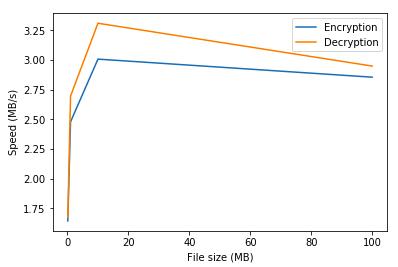
\includegraphics[scale=0.45]{./enc_dec_speed_idea_ecb.png}
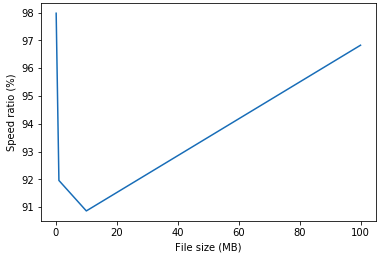
\includegraphics[scale=0.45]{./avg_speed_ratio_idea_ecb.png}
\end{center}
Finally, we repeat this procedure for IDEA in CBC mode, obtaining the following results :
\begin{center}
\begin{tabular}{| c | c | c | c |}
\hline
\multicolumn{4}{|c|}{IDEA-CBC} \\
\hline
File & Encryption (MB/s) & Decryption (MB/s) & Speed ratio\\
\hline
file1.txt & 2.8745 & 3.2579 & 0.8823 \\
\hline
file10.txt & 2.8484 & 3.3236 & 0.8570 \\
\hline
file100.txt & 2.7414 & 3.0032 & 0.9128 \\
\hline
\end{tabular}
\end{center}
\begin{center}
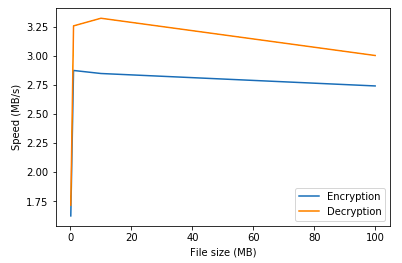
\includegraphics[scale=0.4]{./enc_dec_speed_idea_cbc.png}
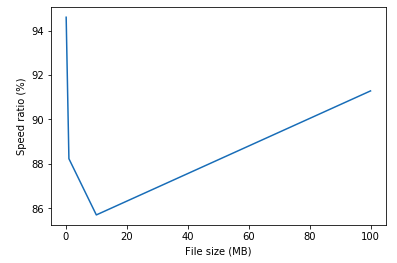
\includegraphics[scale=0.4]{./avg_speed_ratio_idea_cbc.png}
\end{center}
\section{Conclusions}
As we could seen the environment has optimal performances only when our file has a particular size (it falls in an optimal range), in order to divide the work for encryption and decryption processes among threads available. Naturally, when the file size is below or above this range, threads are not exploited as possible in the first case; in the second case, there is too much work for the threads, so the environment wait for one or more thread to finish their current work, in order to assign again a new work. In both cases, we can see from the previous plots that the performance decreases a lot. This experiment is a good mental exercise to start thinking how ciphers and mode of operations are correlated in the cryptography world.
\end{document}